\cleardoublepage

\chapter{Presupuesto}

\section{Componentes hardware y software}

Para la realización de este proyecto no se ha usado dispositvos hardware dedicados como podría ser un Arduino o Raspberry.
Simplemente se ha virtualizado el entorno de pruebas mediante software de vitualización (VirtualBox) y por tanto no ha tenido
coste económico ninguno. En cuanto al software, tampoco se han usado programas con licencias ya que tanto el cliente MQTT 
(mosquitto), la API de SSL y el entorno de desarrollo (Visual Studio Code) son de código libre.

\section{Diagrama de Gantt}

\begin{figure}[H]
    \centering
    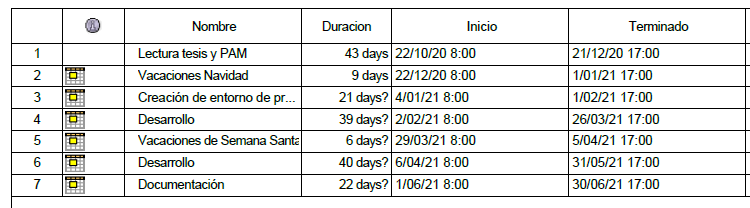
\includegraphics{diagrama-gantt.png}
    \caption{Diagrama de Gantt}
\end{figure}
